%! Author = ASUS
%! Date = 3/6/2023

% Preamble
\documentclass[11pt]{article}

% Packages
\usepackage{amsmath}
\usepackage{wasysym}
\usepackage{graphicx}

% Document
\begin{document}
    \section{Pinhole Camera}

    A pinhole camera is, basically, consists of a small hole and a plane behind. The light from the real world
    object passes through the hole and forms an inverted and laterally inverted image on the plane which is at
    a distance F from the hole. For the sake of simplicity, it is assumed that there is a virtual screen in front
    of the hole at the same distance F. The same image from the real screen is excepted which is upright if the
    image falls on this virtual screen. The distance between the camera's center and the image plane is known
    as the focal length. The intersection of the optical axis of the lens and the image plane is the principal point.
    These parameters, which characterize the internal geometry of the camera, are known as intrinsic parameters.

    #TODO pinhole_2.PNG

    Cameras can have different focal lengths along x and y axes(f_x, f_y). And, principal point (c_x, c_y) are
    the coordinates of the optical center in the image plane.

    Extrinsic parameters describe how the camera is positioned and oriented in relation to the real world frame.
    The translation \mathbf{t} and rotation \mathbf{R} matrices, and scaling of the camera are some of these parameters.

    a 3D point, is projected onto the image plane, by transforming the point from world coordinate system to
    the camera coordinate system using the extrinsic parameters (Rotation \mathbf{R} and Translation \mathbf{t}).
    After having the coordinates of the 3D point from the center of the camera, using the intrinsic parameters
    of the camera, the point is projected onto the image plane. This transformation from world frame to image plane
    is encapsulated in projection matrix.
    #TODO: projection_mat.png


    \section{Stereo Cameras}

    \paragraph{Epipolar geometry}, refers to the geometry of two images of a 3D scene taken
    by two cameras. The two cameras are presumed to have a defined relative pose, which is
    the position and orientation of one camera in relation to the other, and a known internal calibration
    (i.e., focal length, main point). Two geometric primitives, epipolar lines and epipoles, can be used
    to depict the stereo pair's epipolar geometry.
    \paragraph{Epipolar lines:} Any point in one image must lie on the epipolar line for its equivalent
    point in the other image. The intersection of the other camera's picture plane with the plane defined
    by the centers of the two cameras and the point in the first image forms the epipolar line.

    \paragraph{Epipoles:} The epipole is the location where the picture planes of the two cameras are
    intersected by the baseline, which connects the centers of the two cameras. To put it another way,
    each camera perceives the epipole of the other camera as a projection of the other camera's center.
    
    \paragraph{Essential Matrix:} A 3x3 matrix that relates two cameras' poses of two viewpoints. It encodes,
    the relative position and orientation of the two cameras in relation to one another.
    #TODO: E=t'R

    For two identical points p in the first image and p' in the second image, the following equation holds:
    #TODO: pEp' = 0

    By having a set of corresponded points between two images, and the linear equations above, essential matrix
    can be calculated. The most common used algorithm to find the essential matrix is known as "Eight-point algorithm".

    The relative position and orientation of the two cameras, also known as the rotation matrix R and translation
    vector t, can be extracted from the essential matrix once it has been computed.
    
    \paragraph{Fundamental Matrix:} A 3x3 matrix that contains not only relative camera poses but also
    camera intrinsic parameters. It connects corresponding points in the two views to the other view's
    corresponding epipolar lines:
    #TODO: l' = F * p


    By having Essential matrix, K and K' as intrinsic camera matrices, the relation between the matrices is as follows:
    #TODO: F = K' * E * K^-1

    \section{Two View Geometry}

    \paragraph{Two-view geometry} is about finding the of the connection between two images of captured from the same scene
    by two cameras with different viewpoints, and detecting the 3D position of points in the scene.
    Let disparity be the difference in the coordinates of a pixel in the two images. it can be used to calculate
    the depth of the pixel.

    Starting with two cameras with the same intrinsic parameters with parallel baseline, i.e. the planes of
    two cameras are aligned in one line as shown in the following picture, By using similar triangles equations,
    the depth of a keypoint can be calculated:
    #TODO: images and equations

    For other camera settings, e.g. non-parallel baselines, different cameras parameters, The fundamental matrix
    is the key concept that can be used to compute the epipolar lines. Epipolar lines are the intersection of
    the image planes with a plane that passes through the two camera centers and a 3D point in the scene.
    There are several techniques for computing the fundamental matrix, such as the eight-point algorithm.
    Once the fundamental matrix is known, it can be used to compute the essential matrix, which relates the
    two views and the camera internal parameters.

    \paragraph{Reconstructing a scene's 3D structure} from two views is another part of two view geometry.
    A 3D point can be defined as the intersection of the rays that start from the centers of cameras and
    cross corresponded keypoints in each image plane. So, by having the two camera poses (E and F matrices),
    and the coordinates of the same keypoints, the position of the 3D point can be calculated. This process
    is also known as triangulation.

    In practice, first, the essential matrix is calculated by finding the required feature matches between
    to images. Then, for dense reconstruction, the disparity of all pixels along the epipolar lines must be
    calculated. The epipolar lines help to limit the search space for matching features between the two images
    from pixels in all over the images to the epipolar line and its surroundings. By having camera poses and all
    matches, 3D points could be obtained by triangulation.

    \section{Camera Distortion and Calibration}

    \paragraph{Distortion} refers to the deviation between the ideal pinhole camera model and the actual camera
    used to capture images. The pinhole camera model assumes that light rays pass through a single point, or
    the pinhole, before forming an image on a flat image plane. However, real-world cameras have imperfect
    lenses, that causes distortions to the image.

    There are two kinds of camera distortions:

    \begin{enumerate}
        \item Radial distortion is caused by the curvature of the camera lens. This type of distortion
        causes straight lines to appear curved in the image, especially near the edges of the image.
        \item Tangential distortion occurs when the lens is not aligned perfectly parallel to the image plane.
        This causes the image to appear skewed, with some parts appearing closer or farther from the camera
        than they should.
    \end{enumerate}
    {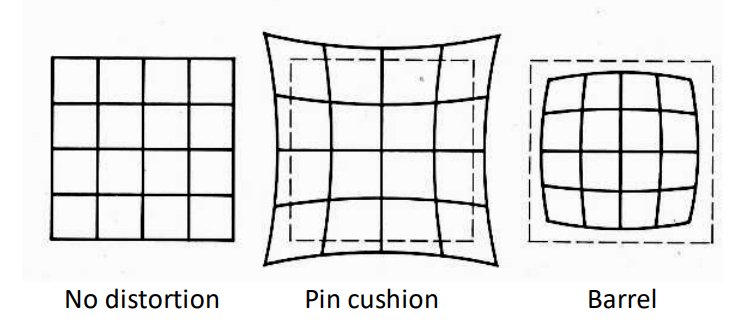
\includegraphics[scale=0.15]{distortion.PNG}}

    \paragraph{Camera calibration} is defined as estimating the intrinsic parameters like focal length,
    principal point, and distortion coefficients, as well as the extrinsic parameters like camera position
    and orientation for each image or frame. The accuracy of this step has significant impact on 3D reconstruction.
    As it is mentioned in previous sections, the depth of a pixel has direct relation with focal length. The depth
    can be in meters, while focal length is usually around millimeters. Therefore, a small error in focal length
    can cause high misplacement of a 3D point.

    Here is a brief general idea of Zhang's method for calibration.
    \paragraph{Homography:} Let there be two images from the same planar scene, e.g. an identity card, but from
    different viewpoints. The second view can be obtained from the first view by multiplying the first image by
    a 3x3 matrix called Homography matrix.


    The goal of the calibration process is to find the 3x3 matrix K, the 3x3 rotation matrix \mathbf{R}, and
    the 3x1 translation vector \mathbf{t} using a set of known 3D points (X_w, Y_w, Z_w) and their corresponding
    image coordinates (u, v).

%    Once the features are detected and matched, the next step is to calibrate the camera parameters

\end{document}
